\documentclass[polish, 11pt, a4paper]{article}

\usepackage{polski}
\usepackage[utf8]{inputenc}
\usepackage[autostyle]{csquotes}
\DeclareQuoteAlias{dutch}{polish}
\usepackage[T1]{fontenc}
\usepackage{geometry}
\geometry{
	a4paper,
	total={170mm,257mm},
	left=25mm,
	right=25mm,
	top=20mm,
}

\usepackage{babel}
\usepackage{microtype}
\usepackage{lmodern}
\usepackage{multirow}
\usepackage{makecell}
\usepackage{array}
\newcolumntype{?}[1]{!{\vrule width #1}}
\usepackage{amsmath}
\usepackage{caption}
\usepackage{graphicx}
\usepackage{graphics}
\usepackage{float}
\usepackage{enumitem}
\usepackage{ragged2e}
\usepackage{parskip}
\RaggedRightParindent = 24 pt
\usepackage{indentfirst}
\usepackage[figurename=Wykres]{caption}

\begin{document}
	\begin{titlepage}
	\centering
	\Huge Laboratorium Podstaw Fizyki\\
	\vspace{1cm}
	\huge Ćwiczenie 20 \enquote{Skalowanie termopary i wyznaczanie temperatury krzepnięcia stopu}\\
	\vspace{1cm}
	\raggedright
	\huge Prowadzący: mgr Karolina Paradowska\\
	\vspace{.5cm}
	\begin{table}[h]
		\centering
		\resizebox{\columnwidth}{!}{%
		\begin{tabular}{|r|l|}\hline
			Imię i Nazwisko	&Marcin Kotas\\\hline
			Nr indeksu		&235098\\\hline
			Wydział			&Elektroniki\\\hline
			Termin zajęć	&14.11.2017, godz. 9.15\\\hline
			Numer grupy ćwiczeniowej&5\\\hline
			Data oddania sprawozdania&21.11.2017\\\hline
		\end{tabular}%
		}
	\end{table}
	\end{titlepage}
	\section{Wstęp teoretyczny}
		\RaggedRight
		Pierwszym celem ćwiczenia było poznanie zasady działania termopary - jej skalowanie oraz wyznaczanie jej współczynnika termoelektrycznego.
		Zależność napięcia od temperatury termopary opisana jest następującym wzorem:
		\begin{equation}
			U=\alpha(T-T_0)
		\end{equation}
		gdzie: \(U\) - napięcie, \(\alpha\) - współczynnik termoelektryczny, \(T\) - temperatura badana, \(T_0\) - temperatura odniesienia (zwykle \(0^\circ C\)).
		
		\begin{figure}[H]
			\centering
			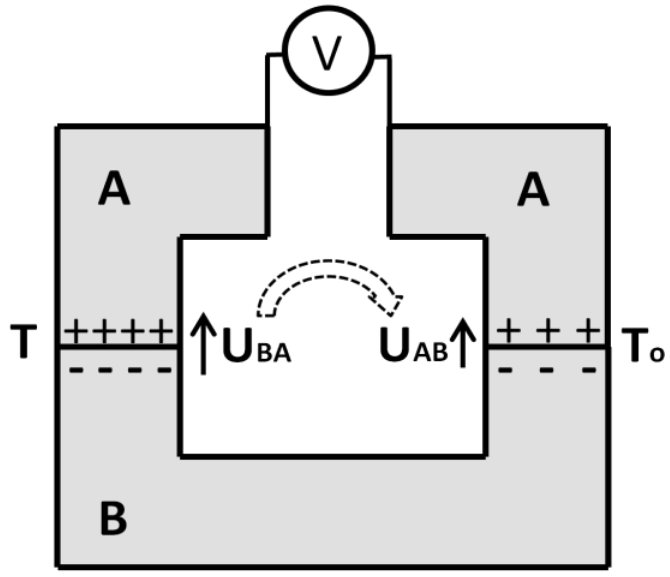
\includegraphics[width=.5\textwidth]{Fizyka20Rysunek1}
			
			Rysunek 1: Schemat przedstawiający zasadę działania termopary. Metal A posiada większą koncentrację elektronów swobodnych niż B, przez co powstaje kontaktowa różnica potencjałów \(U_{BA}\) - zależy ona od temperatury, więc jeśli \(T\neq T_0\) to w obwodzie tworzy się różnica napięć mierzona woltomierzem.
		\end{figure}
		
		Drugim celem było badanie zjawiska krzepnięcia poprzez wyznaczanie temperatury krzepnięcia stopu Wooda.
		Dokładny opis przeprowadzenia pomiarów został opisany w sekcji 2.1 \enquote{Wykonanie pomiarów}.
	\section{Wyniki pomiarów}
		
	\subsection{Wykonanie pomiarów}
		Najpierw przeprowadzone zostało skalowanie termopary. Jedno spojenie termopary umieszczone zostało w termosie z wodą z lodem o temp. \(\sim 0^\circ C\), a drugie w garnku z wodą o temp. \(\sim 16^\circ C\). Garnek z wodą był podgrzewany do osiągnięcia temp. \(90^\circ C\). Napięcie na termoparze zapisywane było co \(2^\circ C\). Wyniki pomiarów zostały umieszczone w Tabeli 1.
		
		Następnie wyznaczona została temperatura krzepnięcia stopu Wooda. Rozgrzany do \(\sim 85^\circ C\) tygiel ze stopem metali został umieszczony na metalowej podstawce. Jedno spojenie termopary pozostało w termosie, a drugie umieszczone zostało w tyglu. Napięcie na termoparze zapisywane było co \(30s\) aż spadło do wartości odpowiadającej \(40^\circ C\). Wyniki zostały umieszczone w Tabeli 2.
	\subsection{Obliczenia}
	
	\subsubsection{Skalowanie termopary}
		Najpierw sporządzony został wykres cechowania termopary (Wykres 1). Dla kilku punktów narysowane zostały słupki błędów. Np. dla \(32^\circ C\) \(u(T)=0,8^\circ C\), \(u(U)=0,002mV\).
		
		Dokładności pomiarów zostały obliczone korzystając ze specyfikacji termometru oraz woltomierza. Dla pomiarów w temperaturze \(30^\circ C\):
		\begin{align*}
		\Delta T&=\pm(0,75\%rdg+1^\circ C) = 0,0075\cdot 30 + 1 = 1,225 [^\circ C]\\
		\Delta U&=\pm(0,05\%rdg+0,01\% \text{pełnej skali}) = 0,0005\cdot 1,499 + 0,0001\cdot 10 = 1,7495\times 10^{-3} [mV]
		\end{align*}
		Niepewności tych pomiarów to niepewności typu B. Wyniki zostały zaokrąglone do rozdzielczości przyrządów pomiarowych:
		\begin{align*}
		u(T)&= \frac{\Delta T}{\sqrt{3}} = \frac{1,225}{\sqrt{3}} = 0,70725408 \approx 0,8 [^\circ C]\\[10pt]
		u(U)&= \frac{\Delta U}{\sqrt{3}} = \frac{0,0017495}{\sqrt{3}} = 0,001010074 \approx 0,002 [mV]
		\end{align*}
		
		Następnie metodą regresji liniowej wyznaczony został współczynnik \(A\) prostej najlepiej dopasowanej do wykresu. 
		Jest to jednocześnie współczynnik termoelektryczny \(\alpha\):
		\begin{align*}
			\alpha 		= A		&= 0,05328[mV/^\circ C]\\
			u(\alpha) 	= u(A)	&= 0,00012[mV/^\circ C]
		\end{align*}
		
	\subsubsection{Wyznaczenie temperatury krzepnięcia stopu Wooda}
		Najpierw sporządzony został wykres zależności napięcia od czasu schładzania stopu (Wykres 2). Napięcie krzepnięcia zostało wyznaczone jako średnia napięć w okresie od 5 do 12 minuty:
		\begin{displaymath}
			U_k=\frac{\sum_{t=5}^{12}U_t}{15}=3,4303[mV]
		\end{displaymath}
		Niepewność standardowa typu A wyznaczonego napięcia wynosi:
		\begin{align*}
		u_A(U_k)&=\sqrt{\frac{\sum_{t=5}^{12} (U_{t}-U_k)^2}{15(15-1)}}\\
		&=\sqrt{\frac{(3,435-3,4303)^2+(3,438-3,4303)^2+\dots+(3,435-3,4303)^2}{210}}\\
		&=0,001713995\approx 0,0018 [mV]
		\end{align*}
		Niepewność standardowa typu B została obliczona jako wartość średnia niepewności napięć:
		\begin{displaymath}
			u_B(U_k) = \frac{\sum_{t=5}^{12}u(U_t)}{15}=0,002[mV]
		\end{displaymath} 
		Końcowa niepewność została obliczona ze wzoru:
		\begin{displaymath}
			u(U_k)	=\sqrt{u_A^2(U_k)+u_B^2(U_k)}=\sqrt{0,0018^2+0,002^2} \approx 0,0027[mV]
		\end{displaymath}
		Temperaturę krzepnięcia można wyznaczyć dzieląc napięcie krzepnięcia przez współczynnik termoelektryczny:
		\begin{displaymath}
			T_k=\frac{U_k}{\alpha}=\frac{3,4303}{0,05328} \approx 64,38[^\circ C]
		\end{displaymath}
		Niepewność wyznaczonej temperatury jest niepewnością złożoną:
		\begin{align*}
		u_c(T_k)	&=\sqrt{\left(\frac{\partial T_k}{\partial U_k}\right)^2\cdot u^2(U_k)+\left(\frac{\partial T_k}{\partial \alpha}\right)^2\cdot u^2(\alpha)}\\
		&=\sqrt{\left(\frac{1}{\alpha}\right)^2\cdot u^2(U_k) + \left(-\frac{U_k}{\alpha^2}\right)^2\cdot u^2(\alpha)}\\
		&=\sqrt{\left(\frac{1}{0,05328}\right)^2\cdot 0,0027^2+\left(-\frac{3,4303}{0,05328^2}\right)^2\cdot 0,00012^2}\\[10pt]
		&=0,14815138\approx 0,15[^\circ C]
		\end{align*}
		
		Wyliczona temperatura nie zgadza się z temperaturą odpowiadającą napięciu \(3,4303mV\) w Tabeli 1 - zgodnie z tabelą \(T_k\approx 66^\circ C\). Błąd wynika z tego, że temperatura wody w termosie była nieco wyższa niż \(0^\circ C\) - przedłużenie wyznaczonej linii trendu przecina poziomą oś w punkcie \(T_0\neq 0^\circ C\). Temperaturę tę można obliczyć ze wzoru wyznaczonej linii trendu:
		\begin{align*}
			0	&=	A\cdot T_0 + B\\[4pt]
			T_0	&=	\frac{-B}{A} = \frac{0,08327}{0,05328} = 1,5628 \approx 1,56 [^\circ C]
		\end{align*}
		Niepewność temperatury odniesienia to niepewność złożona:
		\begin{align*}
		u(T_0)	&=\sqrt{\left(\frac{\partial T_0}{\partial A}\right)^2\cdot u^2(A)+\left(\frac{\partial T_0}{\partial B}\right)^2\cdot u^2(B)}\\
		&=\sqrt{\left(\frac{B}{A^2}\right)^2\cdot u^2(A) + \left(-\frac{1}{A}\right)^2\cdot u^2(B)}\\
		&=\sqrt{\left(\frac{-0,08327}{0,05328^2}\right)^2\cdot 0,00012^2 + \left(-\frac{1}{0,05328}\right)^2\cdot 0,00655^2}\\[10pt]
		&=0,122997\approx 0,13[^\circ C]
		\end{align*}
		Wynik należy uwzględnić w wyznaczaniu temperatury krzepnięcia poprzez przekształcenie wzoru (1):
		\begin{align*}
		U	&=\alpha(T-T_0)\\[4pt]
		T_{k}^+	&=\frac{U_k}{\alpha}+T_0 = T_k + T_0\\[4pt]
		T_{k}^+	&=64,38 + 1,56 = 65,94 [^\circ C]
		\end{align*}
		Niepewność temperatury z poprawką to niepewność złożona:
		\begin{align*}
			u_c(T_k^+)	&=\sqrt{\left(\frac{\partial T_k^+}{\partial T_k}\right)^2\cdot u^2(T_k)+\left(\frac{\partial T_k^+}{\partial T_0}\right)^2\cdot u^2(T_0)}\\[4pt]
			&=\sqrt{1^2\cdot u^2(T_k) +1^2\cdot u^2(T_0)}
			 =\sqrt{0,15^2 + 0,13^2}\\[4pt]
			&=0,198494\approx 0,20[^\circ C]
		\end{align*}
		
	\newpage
	\subsection{Tabele i wykresy}
		\begin{table}[H]
			\begin{minipage}{.5\textwidth}
				\caption{Skalowanie termopary}
				\centering
				\begin{tabular}{|c|c|c|c|}\hline
					\(T\)	&	\(u(T)\) 	&	\(U\) 	&	\(u(U)\) 	\\
					\([^\circ C]\)	&	\([^\circ C]\)	&	\([mV]\)	&	\([mV]\)	\\\hline
					15,6	&	0,7	&	0,784	&	0,001	\\\hline
					16,0	&	0,7	&	0,811	&	0,001	\\\hline
					18,0	&	0,7	&	0,904	&	0,001	\\\hline
					20,0	&	0,7	&	1,006	&	0,001	\\\hline
					22,0	&	0,7	&	1,094	&	0,001	\\\hline
					24,0	&	0,7	&	1,172	&	0,001	\\\hline
					26,0	&	0,7	&	1,290	&	0,001	\\\hline
					28,1	&	0,7	&	1,409	&	0,001	\\\hline
					30,0	&	0,8	&	1,499	&	0,002	\\\hline
					32,0	&	0,8	&	1,602	&	0,002	\\\hline
					34,0	&	0,8	&	1,716	&	0,002	\\\hline
					36,0	&	0,8	&	1,832	&	0,002	\\\hline
					38,0	&	0,8	&	1,947	&	0,002	\\\hline
					40,0	&	0,8	&	2,049	&	0,002	\\\hline
					42,0	&	0,8	&	2,143	&	0,002	\\\hline
					44,0	&	0,8	&	2,245	&	0,002	\\\hline
					46,0	&	0,8	&	2,360	&	0,002	\\\hline
					48,0	&	0,8	&	2,470	&	0,002	\\\hline
					50,0	&	0,8	&	2,578	&	0,002	\\\hline
					52,0	&	0,9	&	2,664	&	0,002	\\\hline
					54,0	&	0,9	&	2,771	&	0,002	\\\hline
					56,0	&	0,9	&	2,890	&	0,002	\\\hline
					58,0	&	0,9	&	3,003	&	0,002	\\\hline
					60,0	&	0,9	&	3,112	&	0,002	\\\hline
					62,0	&	0,9	&	3,216	&	0,002	\\\hline
					64,0	&	0,9	&	3,312	&	0,002	\\\hline
					66,0	&	0,9	&	3,426	&	0,002	\\\hline
					68,0	&	0,9	&	3,537	&	0,002	\\\hline
					70,0	&	0,9	&	3,636	&	0,002	\\\hline
					72,0	&	0,9	&	3,756	&	0,002	\\\hline
					74,0	&	0,9	&	3,856	&	0,002	\\\hline
					76,0	&	1,0	&	3,972	&	0,002	\\\hline
					78,0	&	1,0	&	4,072	&	0,002	\\\hline
					80,0	&	1,0	&	4,189	&	0,002	\\\hline
					82,1	&	1,0	&	4,314	&	0,002	\\\hline
					84,0	&	1,0	&	4,408	&	0,002	\\\hline
					86,0	&	1,0	&	4,510	&	0,002	\\\hline
					88,0	&	1,0	&	4,610	&	0,002	\\\hline
					90,0	&	1,0	&	4,736	&	0,002	\\\Xhline{3\arrayrulewidth}
					\multicolumn{1}{|r}{\(\alpha\)}	&	\([mV/^\circ C]\)	&	\multicolumn{2}{l|}{0,05328}	\\\hline
					\multicolumn{1}{|r}{\(u(\alpha)\)}	&	\([mV/^\circ C]\)	&	\multicolumn{2}{l|}{0,00012}	\\\hline
					\multicolumn{1}{|r}{\(\frac{u(\alpha)}{\alpha}\)}	&	\([\%]\)	&	\multicolumn{2}{l|}{0,23}	\\\hline
				\end{tabular}
			\end{minipage}%
			\begin{minipage}{.5\textwidth}
				\caption{Krzepnięcie stopu}
				\centering
				\begin{tabular}{|c|c|c|}\hline
					\(t\)	&	\(U\) 	&	\(u(U)\) 	\\
					\([min]\)	&	\([mV]\)	&	\([mV]\)	\\\hline
					0,0	&	4,406	&	0,002	\\\hline
					0,5	&	4,242	&	0,002	\\\hline
					1,0	&	4,102	&	0,002	\\\hline
					1,5	&	3,973	&	0,002	\\\hline
					2,0	&	3,850	&	0,002	\\\hline
					2,5	&	3,730	&	0,002	\\\hline
					3,0	&	3,618	&	0,002	\\\hline
					3,5	&	3,526	&	0,002	\\\hline
					4,0	&	3,463	&	0,002	\\\hline
					4,5	&	3,437	&	0,002	\\\hline
					5,0	&	3,435	&	0,002	\\\hline
					5,5	&	3,438	&	0,002	\\\hline
					6,0	&	3,440	&	0,002	\\\hline
					6,5	&	3,438	&	0,002	\\\hline
					7,0	&	3,434	&	0,002	\\\hline
					7,5	&	3,429	&	0,002	\\\hline
					8,0	&	3,426	&	0,002	\\\hline
					8,5	&	3,424	&	0,002	\\\hline
					9,0	&	3,420	&	0,002	\\\hline
					9,5	&	3,421	&	0,002	\\\hline
					10,0	&	3,423	&	0,002	\\\hline
					10,5	&	3,426	&	0,002	\\\hline
					11,0	&	3,430	&	0,002	\\\hline
					11,5	&	3,435	&	0,002	\\\hline
					12,0	&	3,435	&	0,002	\\\hline
					12,5	&	3,396	&	0,002	\\\hline
					13,0	&	3,355	&	0,002	\\\hline
					13,5	&	3,313	&	0,002	\\\hline
					14,0	&	3,257	&	0,002	\\\hline
					14,5	&	3,140	&	0,002	\\\hline
					15,0	&	2,918	&	0,002	\\\hline
					15,5	&	2,693	&	0,002	\\\hline
					16,0	&	2,516	&	0,002	\\\hline
					16,5	&	2,380	&	0,002	\\\hline
					17,0	&	2,282	&	0,002	\\\hline
					17,5	&	2,210	&	0,002	\\\hline
					18,0	&	2,156	&	0,002	\\\hline
					18,5	&	2,116	&	0,002	\\\hline
					19,0	&	2,084	&	0,002	\\\hline
					19,5	&	2,060	&	0,002	\\\hline
					20,0	&	2,042	&	0,002	\\\Xhline{3\arrayrulewidth}
					\multicolumn{1}{|r}{\(U_k\)}	&	\([mV]\)	&	3,4303	\\\hline
					\multicolumn{1}{|r}{\(u(U_k)\)}	&	\([mV]\)	&	0,0027	\\\hline
					\multicolumn{1}{|r}{\(T_k^+\)}	&	\([^\circ C]\)	&	65,94	\\\hline
					\multicolumn{1}{|r}{\(u_c(T_k^+)\)}	&	\([^\circ C]\)	&	0,20	\\\hline
					\multicolumn{1}{|r}{\(\frac{u_c(T_k^+)}{T_k^+}\)}	&	\([\%]\)	&	0,30	\\\hline
				\end{tabular}
			\end{minipage}
		\end{table}
	
		\begin{figure}[H]
			\centering
			\caption{Skalowanie termopary}
			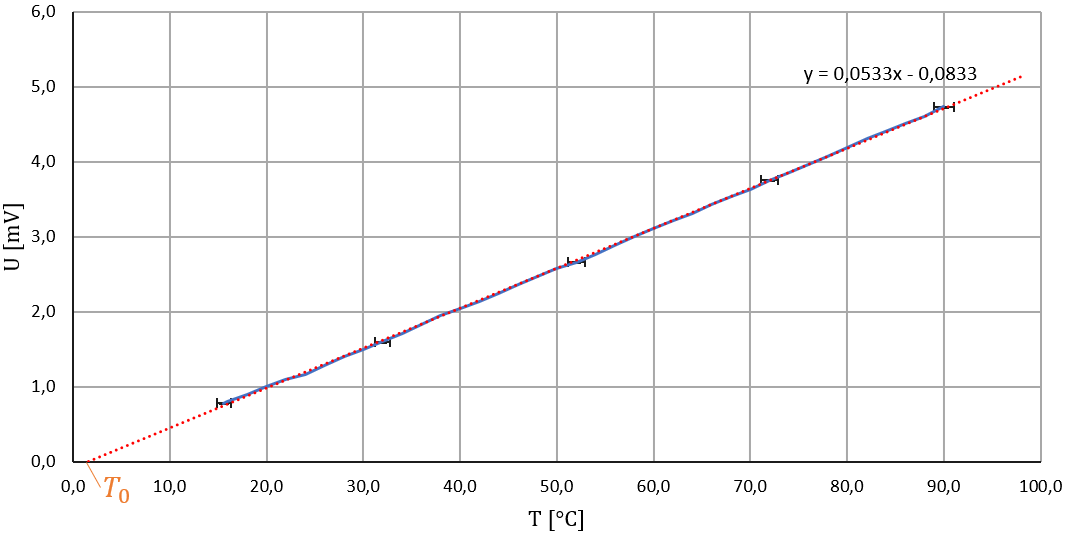
\includegraphics[width=\textwidth]{Fizyka20Wykres1}
		\end{figure}
	
		\begin{figure}[H]
			\centering
			\caption{Krzepnięcie stopu metali}
			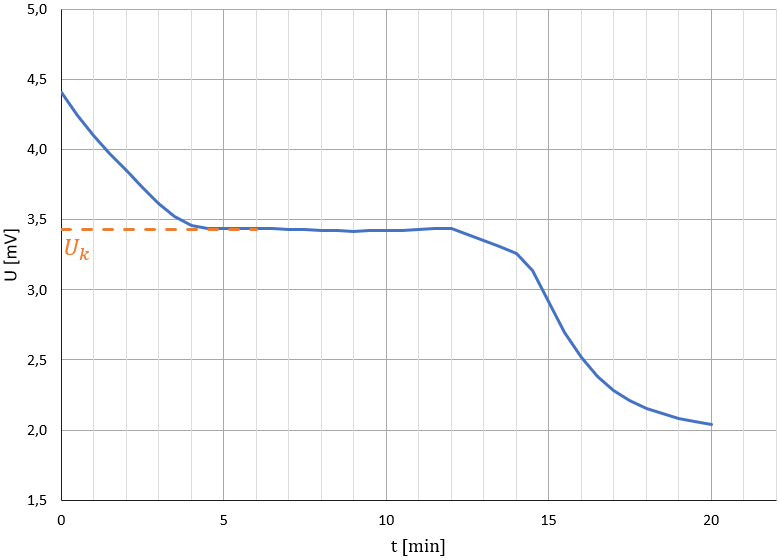
\includegraphics[width=\textwidth]{Fizyka20Wykres2}
		\end{figure}
	
	\newpage
	\section{Ostateczne wyniki}
		Ostateczne wyniki wraz z zaokrągleniami:
		\begin{description}[align=right,labelwidth=8cm]
			\item [Współczynnik termoelektryczny:] {\((0,05328\pm 0,00012)mV/^\circ C\)}
			\item [Napięcie krzepnięcia:] {\((3,4303\pm 0,0027)mV\)}
			\item [Temperatura krzepnięcia:] {\((64,38\pm 0,15)^\circ C\)}
			\item [Temperatura krzepnięcia z poprawką:] {\((65,94\pm 0,20)^\circ C\)}
		\end{description}
	
	\section{Dyskusja i wnioski}
		Współczynnik termoelektryczny został wyznaczony z wysoką dokładnością - błąd względny wyniósł \(0,23\%\). Wynika to z dużej dokładności woltomierza oraz ze starannego i umiejętnego wykonania pomiarów.
		Wyznaczenie temperatury krzepnięcia wymagało wprowadzenia poprawki. Powodem tego była niezerowa temperatura wody w termosie. Wynik uwzględniający poprawkę jest spójny z danymi w literaturze (\(66-70^\circ C\)) Dokładność tego pomiaru również jest bardzo wysoka (błąd względny wynosi \(0,30\%\)).
		
	\section{Literatura}
	\begin{enumerate}[label={[\arabic*]}]
		\item http://delibra.bg.polsl.pl/dlibra/doccontent?id=17399
		\item \enquote{Materials Handbook: A Concise Desktop Reference}, François Cardarelli, str. 210 (źródło: Google Książki )
	\end{enumerate}
\end{document}